If the robot uses the path $p=R_{13},R_{14},R_{15},R_{16},R_{17},R_{20},R_{21},R_{28},R_{33},R_{34},R_{35},R_{36},R_{25},R_{R_24},R_{13}...$ it will go in an infinite loop passing a red state infinite times. Never passing an obstacle and after each time it passes a red state it passes a blue state right after. Se figure \ref{inf_path}
\begin{figure}[H]
 \centering
  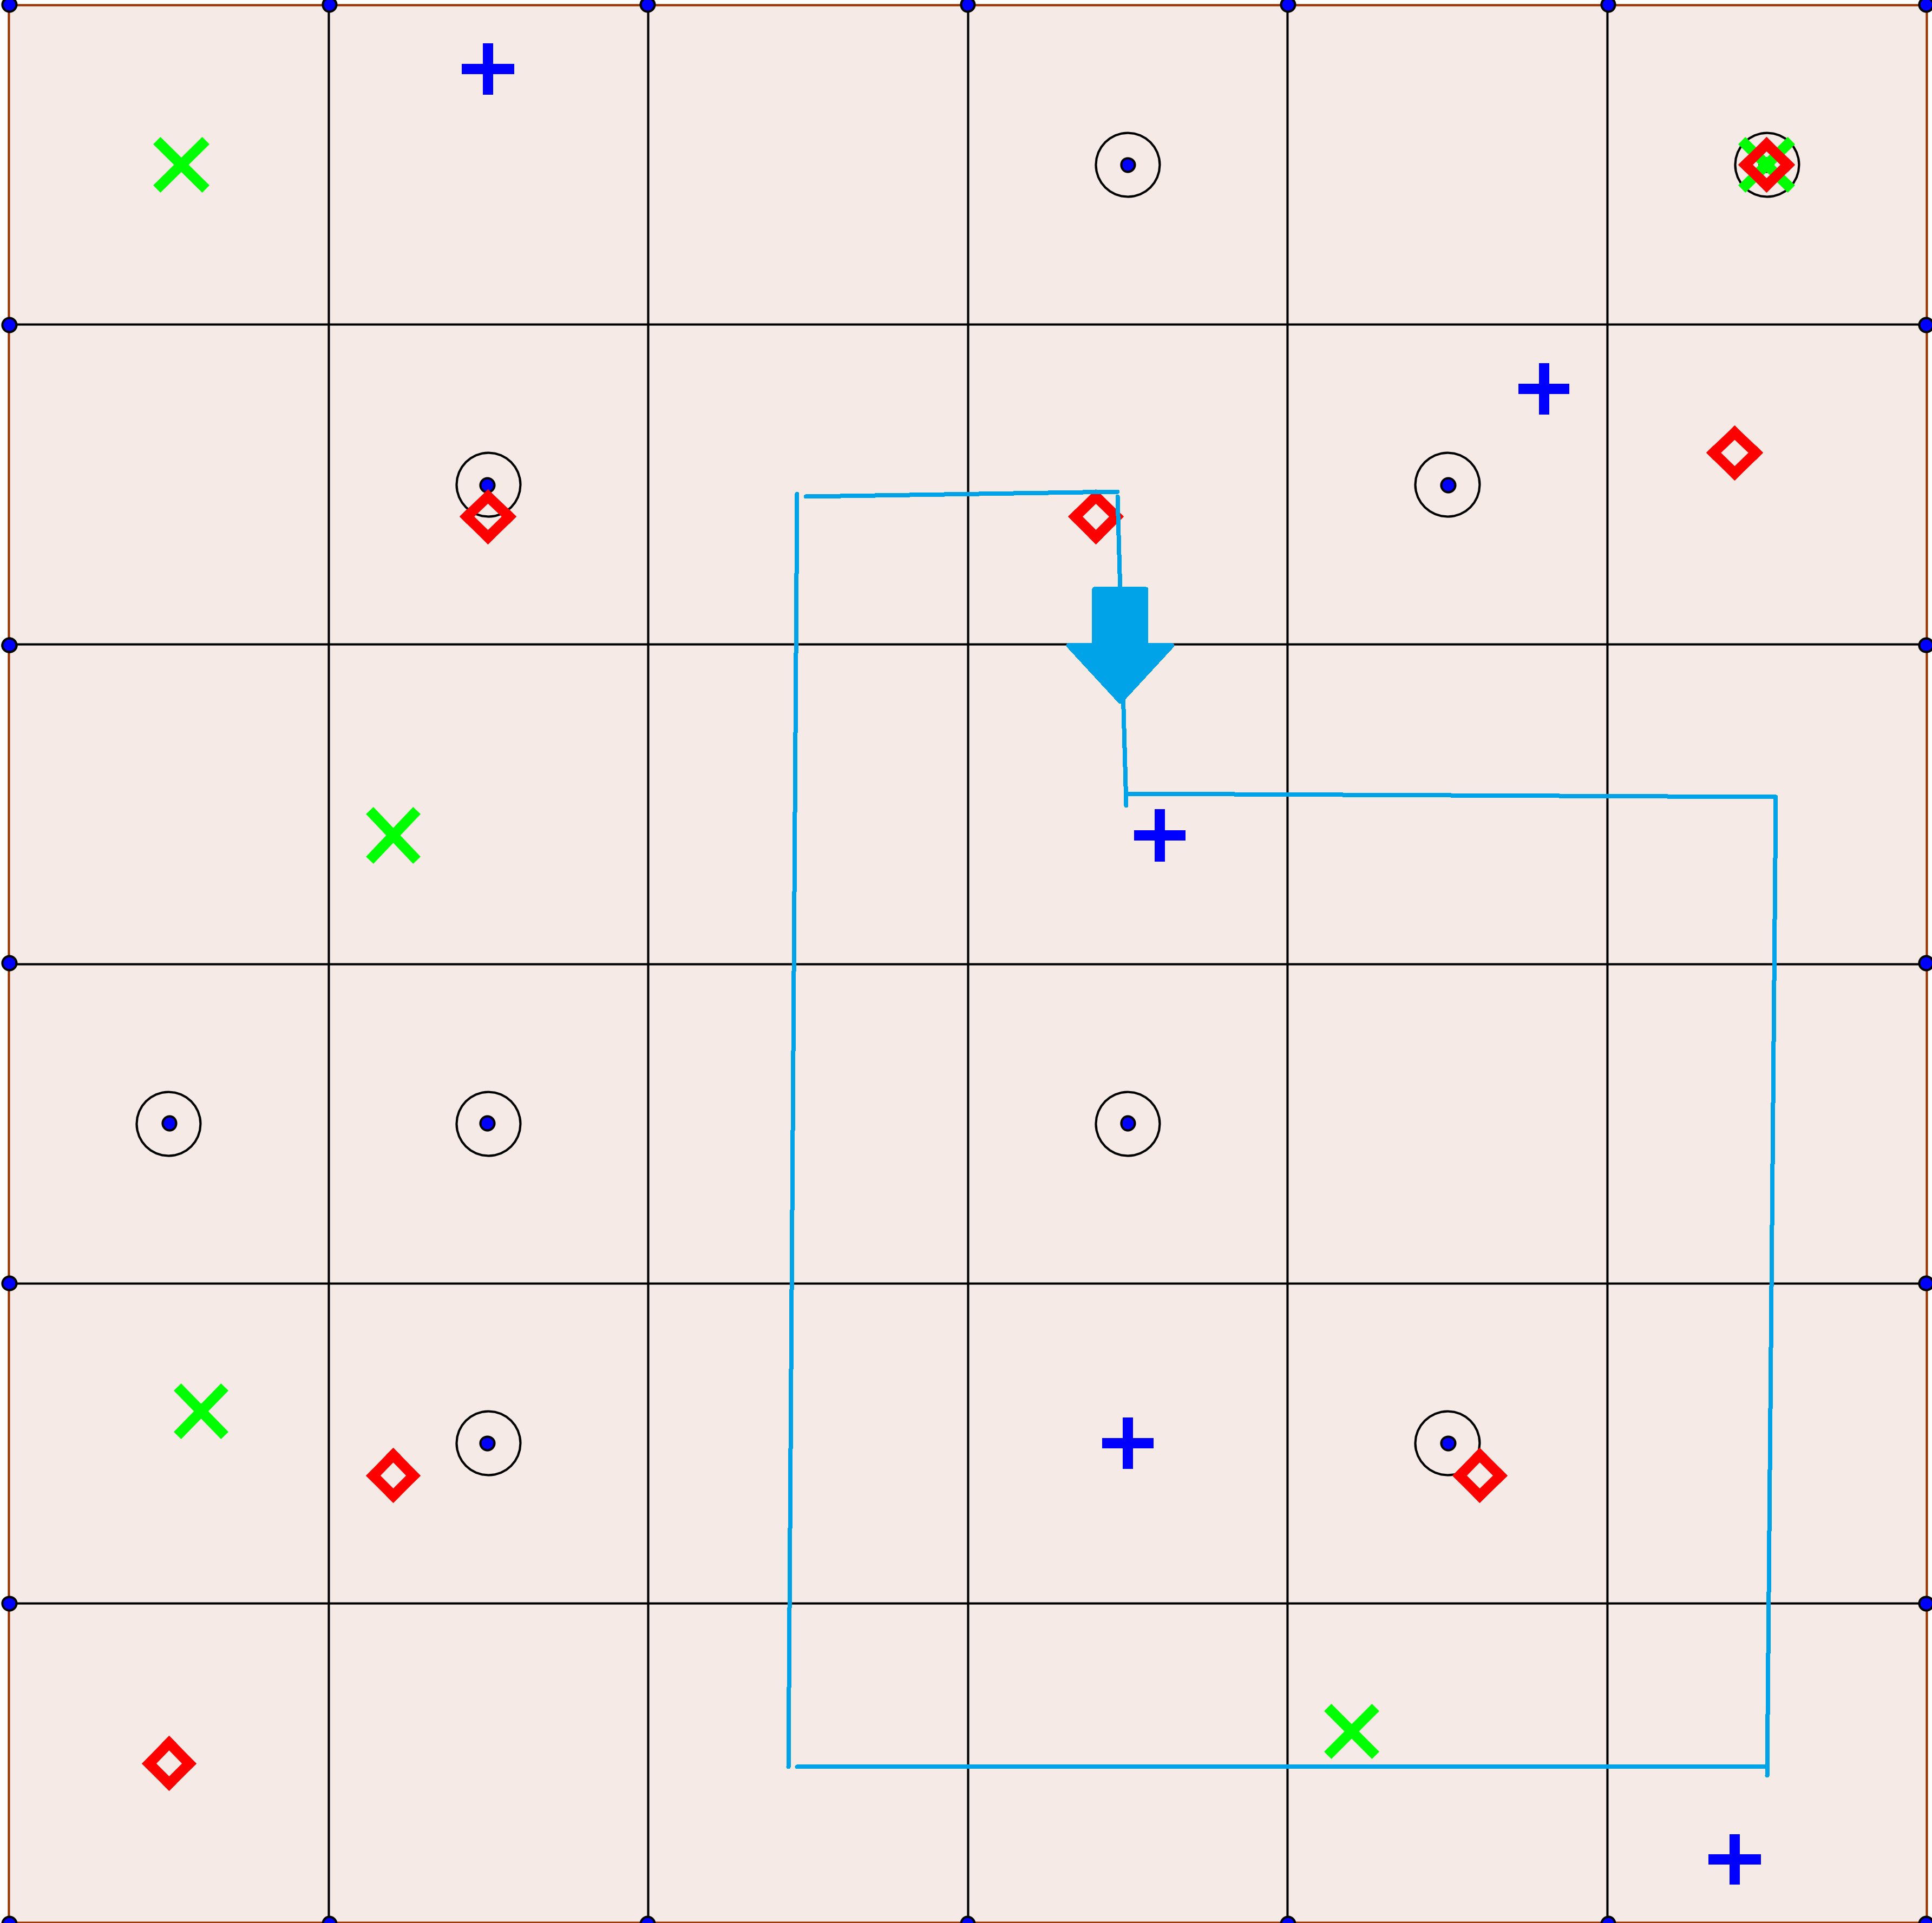
\includegraphics[width = 0.8\textwidth]{hw3_map_path.png}
  \caption{The infinite path}
  \label{inf_path}
  \end{figure}
